% Options for packages loaded elsewhere
\PassOptionsToPackage{unicode}{hyperref}
\PassOptionsToPackage{hyphens}{url}
%
\documentclass[
]{book}
\usepackage{amsmath,amssymb}
\usepackage{lmodern}
\usepackage{ifxetex,ifluatex}
\ifnum 0\ifxetex 1\fi\ifluatex 1\fi=0 % if pdftex
  \usepackage[T1]{fontenc}
  \usepackage[utf8]{inputenc}
  \usepackage{textcomp} % provide euro and other symbols
\else % if luatex or xetex
  \usepackage{unicode-math}
  \defaultfontfeatures{Scale=MatchLowercase}
  \defaultfontfeatures[\rmfamily]{Ligatures=TeX,Scale=1}
\fi
% Use upquote if available, for straight quotes in verbatim environments
\IfFileExists{upquote.sty}{\usepackage{upquote}}{}
\IfFileExists{microtype.sty}{% use microtype if available
  \usepackage[]{microtype}
  \UseMicrotypeSet[protrusion]{basicmath} % disable protrusion for tt fonts
}{}
\makeatletter
\@ifundefined{KOMAClassName}{% if non-KOMA class
  \IfFileExists{parskip.sty}{%
    \usepackage{parskip}
  }{% else
    \setlength{\parindent}{0pt}
    \setlength{\parskip}{6pt plus 2pt minus 1pt}}
}{% if KOMA class
  \KOMAoptions{parskip=half}}
\makeatother
\usepackage{xcolor}
\IfFileExists{xurl.sty}{\usepackage{xurl}}{} % add URL line breaks if available
\IfFileExists{bookmark.sty}{\usepackage{bookmark}}{\usepackage{hyperref}}
\hypersetup{
  pdftitle={A Minimal Book Example},
  pdfauthor={John Doe},
  hidelinks,
  pdfcreator={LaTeX via pandoc}}
\urlstyle{same} % disable monospaced font for URLs
\usepackage{color}
\usepackage{fancyvrb}
\newcommand{\VerbBar}{|}
\newcommand{\VERB}{\Verb[commandchars=\\\{\}]}
\DefineVerbatimEnvironment{Highlighting}{Verbatim}{commandchars=\\\{\}}
% Add ',fontsize=\small' for more characters per line
\usepackage{framed}
\definecolor{shadecolor}{RGB}{248,248,248}
\newenvironment{Shaded}{\begin{snugshade}}{\end{snugshade}}
\newcommand{\AlertTok}[1]{\textcolor[rgb]{0.94,0.16,0.16}{#1}}
\newcommand{\AnnotationTok}[1]{\textcolor[rgb]{0.56,0.35,0.01}{\textbf{\textit{#1}}}}
\newcommand{\AttributeTok}[1]{\textcolor[rgb]{0.77,0.63,0.00}{#1}}
\newcommand{\BaseNTok}[1]{\textcolor[rgb]{0.00,0.00,0.81}{#1}}
\newcommand{\BuiltInTok}[1]{#1}
\newcommand{\CharTok}[1]{\textcolor[rgb]{0.31,0.60,0.02}{#1}}
\newcommand{\CommentTok}[1]{\textcolor[rgb]{0.56,0.35,0.01}{\textit{#1}}}
\newcommand{\CommentVarTok}[1]{\textcolor[rgb]{0.56,0.35,0.01}{\textbf{\textit{#1}}}}
\newcommand{\ConstantTok}[1]{\textcolor[rgb]{0.00,0.00,0.00}{#1}}
\newcommand{\ControlFlowTok}[1]{\textcolor[rgb]{0.13,0.29,0.53}{\textbf{#1}}}
\newcommand{\DataTypeTok}[1]{\textcolor[rgb]{0.13,0.29,0.53}{#1}}
\newcommand{\DecValTok}[1]{\textcolor[rgb]{0.00,0.00,0.81}{#1}}
\newcommand{\DocumentationTok}[1]{\textcolor[rgb]{0.56,0.35,0.01}{\textbf{\textit{#1}}}}
\newcommand{\ErrorTok}[1]{\textcolor[rgb]{0.64,0.00,0.00}{\textbf{#1}}}
\newcommand{\ExtensionTok}[1]{#1}
\newcommand{\FloatTok}[1]{\textcolor[rgb]{0.00,0.00,0.81}{#1}}
\newcommand{\FunctionTok}[1]{\textcolor[rgb]{0.00,0.00,0.00}{#1}}
\newcommand{\ImportTok}[1]{#1}
\newcommand{\InformationTok}[1]{\textcolor[rgb]{0.56,0.35,0.01}{\textbf{\textit{#1}}}}
\newcommand{\KeywordTok}[1]{\textcolor[rgb]{0.13,0.29,0.53}{\textbf{#1}}}
\newcommand{\NormalTok}[1]{#1}
\newcommand{\OperatorTok}[1]{\textcolor[rgb]{0.81,0.36,0.00}{\textbf{#1}}}
\newcommand{\OtherTok}[1]{\textcolor[rgb]{0.56,0.35,0.01}{#1}}
\newcommand{\PreprocessorTok}[1]{\textcolor[rgb]{0.56,0.35,0.01}{\textit{#1}}}
\newcommand{\RegionMarkerTok}[1]{#1}
\newcommand{\SpecialCharTok}[1]{\textcolor[rgb]{0.00,0.00,0.00}{#1}}
\newcommand{\SpecialStringTok}[1]{\textcolor[rgb]{0.31,0.60,0.02}{#1}}
\newcommand{\StringTok}[1]{\textcolor[rgb]{0.31,0.60,0.02}{#1}}
\newcommand{\VariableTok}[1]{\textcolor[rgb]{0.00,0.00,0.00}{#1}}
\newcommand{\VerbatimStringTok}[1]{\textcolor[rgb]{0.31,0.60,0.02}{#1}}
\newcommand{\WarningTok}[1]{\textcolor[rgb]{0.56,0.35,0.01}{\textbf{\textit{#1}}}}
\usepackage{longtable,booktabs,array}
\usepackage{calc} % for calculating minipage widths
% Correct order of tables after \paragraph or \subparagraph
\usepackage{etoolbox}
\makeatletter
\patchcmd\longtable{\par}{\if@noskipsec\mbox{}\fi\par}{}{}
\makeatother
% Allow footnotes in longtable head/foot
\IfFileExists{footnotehyper.sty}{\usepackage{footnotehyper}}{\usepackage{footnote}}
\makesavenoteenv{longtable}
\usepackage{graphicx}
\makeatletter
\def\maxwidth{\ifdim\Gin@nat@width>\linewidth\linewidth\else\Gin@nat@width\fi}
\def\maxheight{\ifdim\Gin@nat@height>\textheight\textheight\else\Gin@nat@height\fi}
\makeatother
% Scale images if necessary, so that they will not overflow the page
% margins by default, and it is still possible to overwrite the defaults
% using explicit options in \includegraphics[width, height, ...]{}
\setkeys{Gin}{width=\maxwidth,height=\maxheight,keepaspectratio}
% Set default figure placement to htbp
\makeatletter
\def\fps@figure{htbp}
\makeatother
\setlength{\emergencystretch}{3em} % prevent overfull lines
\providecommand{\tightlist}{%
  \setlength{\itemsep}{0pt}\setlength{\parskip}{0pt}}
\setcounter{secnumdepth}{5}
\usepackage{booktabs}
\ifluatex
  \usepackage{selnolig}  % disable illegal ligatures
\fi
\usepackage[]{natbib}
\bibliographystyle{plainnat}

\title{A Minimal Book Example}
\author{John Doe}
\date{2021-10-27}

\usepackage{amsthm}
\newtheorem{theorem}{Theorem}[chapter]
\newtheorem{lemma}{Lemma}[chapter]
\newtheorem{corollary}{Corollary}[chapter]
\newtheorem{proposition}{Proposition}[chapter]
\newtheorem{conjecture}{Conjecture}[chapter]
\theoremstyle{definition}
\newtheorem{definition}{Definition}[chapter]
\theoremstyle{definition}
\newtheorem{example}{Example}[chapter]
\theoremstyle{definition}
\newtheorem{exercise}{Exercise}[chapter]
\theoremstyle{definition}
\newtheorem{hypothesis}{Hypothesis}[chapter]
\theoremstyle{remark}
\newtheorem*{remark}{Remark}
\newtheorem*{solution}{Solution}
\begin{document}
\maketitle

{
\setcounter{tocdepth}{1}
\tableofcontents
}
\hypertarget{about}{%
\chapter{About}\label{about}}

This is a \emph{sample} book written in \textbf{Markdown}. You can use anything that Pandoc's Markdown supports; for example, a math equation \(a^2 + b^2 = c^2\).

\hypertarget{usage}{%
\section{Usage}\label{usage}}

Each \textbf{bookdown} chapter is an .Rmd file, and each .Rmd file can contain one (and only one) chapter. A chapter \emph{must} start with a first-level heading: \texttt{\#\ A\ good\ chapter}, and can contain one (and only one) first-level heading.

Use second-level and higher headings within chapters like: \texttt{\#\#\ A\ short\ section} or \texttt{\#\#\#\ An\ even\ shorter\ section}.

The \texttt{index.Rmd} file is required, and is also your first book chapter. It will be the homepage when you render the book.

\hypertarget{render-book}{%
\section{Render book}\label{render-book}}

You can render the HTML version of this example book without changing anything:

\begin{enumerate}
\def\labelenumi{\arabic{enumi}.}
\item
  Find the \textbf{Build} pane in the RStudio IDE, and
\item
  Click on \textbf{Build Book}, then select your output format, or select ``All formats'' if you'd like to use multiple formats from the same book source files.
\end{enumerate}

Or build the book from the R console:

\begin{Shaded}
\begin{Highlighting}[]
\NormalTok{bookdown}\SpecialCharTok{::}\FunctionTok{render\_book}\NormalTok{()}
\end{Highlighting}
\end{Shaded}

To render this example to PDF as a \texttt{bookdown::pdf\_book}, you'll need to install XeLaTeX. You are recommended to install TinyTeX (which includes XeLaTeX): \url{https://yihui.org/tinytex/}.

\hypertarget{preview-book}{%
\section{Preview book}\label{preview-book}}

As you work, you may start a local server to live preview this HTML book. This preview will update as you edit the book when you save individual .Rmd files. You can start the server in a work session by using the RStudio add-in ``Preview book'', or from the R console:

\begin{Shaded}
\begin{Highlighting}[]
\NormalTok{bookdown}\SpecialCharTok{::}\FunctionTok{serve\_book}\NormalTok{()}
\end{Highlighting}
\end{Shaded}

\hypertarget{hello-bookdown}{%
\chapter{Hello bookdown}\label{hello-bookdown}}

All chapters start with a first-level heading followed by your chapter title, like the line above. There should be only one first-level heading (\texttt{\#}) per .Rmd file.

\hypertarget{a-section}{%
\section{A section}\label{a-section}}

All chapter sections start with a second-level (\texttt{\#\#}) or higher heading followed by your section title, like the sections above and below here. You can have as many as you want within a chapter.

\hypertarget{an-unnumbered-section}{%
\subsection*{An unnumbered section}\label{an-unnumbered-section}}
\addcontentsline{toc}{subsection}{An unnumbered section}

Chapters and sections are numbered by default. To un-number a heading, add a \texttt{\{.unnumbered\}} or the shorter \texttt{\{-\}} at the end of the heading, like in this section.

\hypertarget{cross}{%
\chapter{Cross-references}\label{cross}}

Cross-references make it easier for your readers to find and link to elements in your book.

\hypertarget{chapters-and-sub-chapters}{%
\section{Chapters and sub-chapters}\label{chapters-and-sub-chapters}}

There are two steps to cross-reference any heading:

\begin{enumerate}
\def\labelenumi{\arabic{enumi}.}
\tightlist
\item
  Label the heading: \texttt{\#\ Hello\ world\ \{\#nice-label\}}.

  \begin{itemize}
  \tightlist
  \item
    Leave the label off if you like the automated heading generated based on your heading title: for example, \texttt{\#\ Hello\ world} = \texttt{\#\ Hello\ world\ \{\#hello-world\}}.
  \item
    To label an un-numbered heading, use: \texttt{\#\ Hello\ world\ \{-\#nice-label\}} or \texttt{\{\#\ Hello\ world\ .unnumbered\}}.
  \end{itemize}
\item
  Next, reference the labeled heading anywhere in the text using \texttt{\textbackslash{}@ref(nice-label)}; for example, please see Chapter \ref{cross}.

  \begin{itemize}
  \tightlist
  \item
    If you prefer text as the link instead of a numbered reference use: \protect\hyperlink{cross}{any text you want can go here}.
  \end{itemize}
\end{enumerate}

\hypertarget{captioned-figures-and-tables}{%
\section{Captioned figures and tables}\label{captioned-figures-and-tables}}

Figures and tables \emph{with captions} can also be cross-referenced from elsewhere in your book using \texttt{\textbackslash{}@ref(fig:chunk-label)} and \texttt{\textbackslash{}@ref(tab:chunk-label)}, respectively.

See Figure \ref{fig:nice-fig}.

\begin{Shaded}
\begin{Highlighting}[]
\FunctionTok{par}\NormalTok{(}\AttributeTok{mar =} \FunctionTok{c}\NormalTok{(}\DecValTok{4}\NormalTok{, }\DecValTok{4}\NormalTok{, .}\DecValTok{1}\NormalTok{, .}\DecValTok{1}\NormalTok{))}
\FunctionTok{plot}\NormalTok{(pressure, }\AttributeTok{type =} \StringTok{\textquotesingle{}b\textquotesingle{}}\NormalTok{, }\AttributeTok{pch =} \DecValTok{19}\NormalTok{)}
\end{Highlighting}
\end{Shaded}

\begin{figure}

{\centering 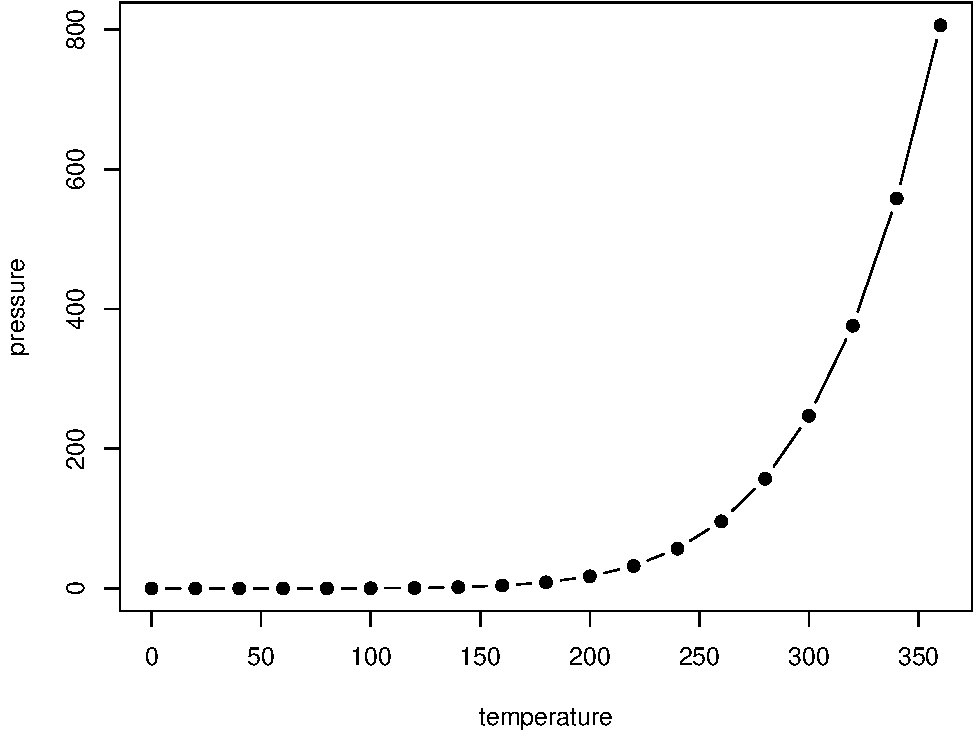
\includegraphics[width=0.8\linewidth]{_main_files/figure-latex/nice-fig-1} 

}

\caption{Here is a nice figure!}\label{fig:nice-fig}
\end{figure}

Don't miss Table \ref{tab:nice-tab}.

\begin{Shaded}
\begin{Highlighting}[]
\NormalTok{knitr}\SpecialCharTok{::}\FunctionTok{kable}\NormalTok{(}
  \FunctionTok{head}\NormalTok{(pressure, }\DecValTok{10}\NormalTok{), }\AttributeTok{caption =} \StringTok{\textquotesingle{}Here is a nice table!\textquotesingle{}}\NormalTok{,}
  \AttributeTok{booktabs =} \ConstantTok{TRUE}
\NormalTok{)}
\end{Highlighting}
\end{Shaded}

\begin{table}

\caption{\label{tab:nice-tab}Here is a nice table!}
\centering
\begin{tabular}[t]{rr}
\toprule
temperature & pressure\\
\midrule
0 & 0.0002\\
20 & 0.0012\\
40 & 0.0060\\
60 & 0.0300\\
80 & 0.0900\\
\addlinespace
100 & 0.2700\\
120 & 0.7500\\
140 & 1.8500\\
160 & 4.2000\\
180 & 8.8000\\
\bottomrule
\end{tabular}
\end{table}

\hypertarget{parts}{%
\chapter{Parts}\label{parts}}

You can add parts to organize one or more book chapters together. Parts can be inserted at the top of an .Rmd file, before the first-level chapter heading in that same file.

Add a numbered part: \texttt{\#\ (PART)\ Act\ one\ \{-\}} (followed by \texttt{\#\ A\ chapter})

Add an unnumbered part: \texttt{\#\ (PART\textbackslash{}*)\ Act\ one\ \{-\}} (followed by \texttt{\#\ A\ chapter})

Add an appendix as a special kind of un-numbered part: \texttt{\#\ (APPENDIX)\ Other\ stuff\ \{-\}} (followed by \texttt{\#\ A\ chapter}). Chapters in an appendix are prepended with letters instead of numbers.

\hypertarget{footnotes-and-citations}{%
\chapter{Footnotes and citations}\label{footnotes-and-citations}}

\hypertarget{footnotes}{%
\section{Footnotes}\label{footnotes}}

Footnotes are put inside the square brackets after a caret \texttt{\^{}{[}{]}}. Like this one \footnote{This is a footnote.}.

\hypertarget{citations}{%
\section{Citations}\label{citations}}

Reference items in your bibliography file(s) using \texttt{@key}.

For example, we are using the \textbf{bookdown} package \citep{R-bookdown} (check out the last code chunk in index.Rmd to see how this citation key was added) in this sample book, which was built on top of R Markdown and \textbf{knitr} \citep{xie2015} (this citation was added manually in an external file book.bib).
Note that the \texttt{.bib} files need to be listed in the index.Rmd with the YAML \texttt{bibliography} key.

The RStudio Visual Markdown Editor can also make it easier to insert citations: \url{https://rstudio.github.io/visual-markdown-editing/\#/citations}

\hypertarget{blocks}{%
\chapter{Blocks}\label{blocks}}

\hypertarget{equations}{%
\section{Equations}\label{equations}}

Here is an equation.

\begin{equation} 
  f\left(k\right) = \binom{n}{k} p^k\left(1-p\right)^{n-k}
  \label{eq:binom}
\end{equation}

You may refer to using \texttt{\textbackslash{}@ref(eq:binom)}, like see Equation \eqref{eq:binom}.

\hypertarget{theorems-and-proofs}{%
\section{Theorems and proofs}\label{theorems-and-proofs}}

Labeled theorems can be referenced in text using \texttt{\textbackslash{}@ref(thm:tri)}, for example, check out this smart theorem \ref{thm:tri}.

\begin{theorem}
\protect\hypertarget{thm:tri}{}\label{thm:tri}For a right triangle, if \(c\) denotes the \emph{length} of the hypotenuse
and \(a\) and \(b\) denote the lengths of the \textbf{other} two sides, we have
\[a^2 + b^2 = c^2\]
\end{theorem}

Read more here \url{https://bookdown.org/yihui/bookdown/markdown-extensions-by-bookdown.html}.

\hypertarget{callout-blocks}{%
\section{Callout blocks}\label{callout-blocks}}

The R Markdown Cookbook provides more help on how to use custom blocks to design your own callouts: \url{https://bookdown.org/yihui/rmarkdown-cookbook/custom-blocks.html}

\hypertarget{sharing-your-book}{%
\chapter{Sharing your book}\label{sharing-your-book}}

\hypertarget{publishing}{%
\section{Publishing}\label{publishing}}

HTML books can be published online, see: \url{https://bookdown.org/yihui/bookdown/publishing.html}

\hypertarget{pages}{%
\section{404 pages}\label{pages}}

By default, users will be directed to a 404 page if they try to access a webpage that cannot be found. If you'd like to customize your 404 page instead of using the default, you may add either a \texttt{\_404.Rmd} or \texttt{\_404.md} file to your project root and use code and/or Markdown syntax.

\hypertarget{metadata-for-sharing}{%
\section{Metadata for sharing}\label{metadata-for-sharing}}

Bookdown HTML books will provide HTML metadata for social sharing on platforms like Twitter, Facebook, and LinkedIn, using information you provide in the \texttt{index.Rmd} YAML. To setup, set the \texttt{url} for your book and the path to your \texttt{cover-image} file. Your book's \texttt{title} and \texttt{description} are also used.

This \texttt{gitbook} uses the same social sharing data across all chapters in your book- all links shared will look the same.

Specify your book's source repository on GitHub using the \texttt{edit} key under the configuration options in the \texttt{\_output.yml} file, which allows users to suggest an edit by linking to a chapter's source file.

Read more about the features of this output format here:

\url{https://pkgs.rstudio.com/bookdown/reference/gitbook.html}

Or use:

\begin{Shaded}
\begin{Highlighting}[]
\NormalTok{?bookdown}\SpecialCharTok{::}\NormalTok{gitbook}
\end{Highlighting}
\end{Shaded}

\hypertarget{cox-regression}{%
\chapter{5. Cox Regression}\label{cox-regression}}

\hypertarget{proportional-hazards-model}{%
\section{Proportional Hazards Model}\label{proportional-hazards-model}}

Proposed by Cox (1972, JRSS-B), primarily to model the relationship between \textbf{hazard function} and \textbf{covariates}. most cited paper in statistics ( 41; 000 as of April 2016), one of the most cited in science.

Several extensions to more complex data structures, e.g., clustered failure time data, or recurrent event data, etc.

※ Data Structure

Observed data: \(\Big \{ X_i = T_i \wedge C_i, \; \; \; \Delta_i = I(T_i < C_i), \; \;\; \mathbf Z_i (\cdot) \Big \} \overset {iid} \sim\)

추가로 \(N_i = I(X_i \le t , \; \Delta_i = 1)\), \(Z_i(t)\) = covariate vector (possibly time-dependent).

\hypertarget{cox-ph-model}{%
\section{Cox PH Model}\label{cox-ph-model}}

\[
\lambda_i (t) = \lambda (t \vert Z_i ) = \lambda_0 (t) \exp (\beta' Z_i) \tag{Cox Model}
\]

semiparametric model:

\begin{itemize}
\tightlist
\item
  \(\exp(\beta ' Z_i)\), parametric assumption on covariate effects
\item
  multiplicative model
\item
  \(\beta\) : \(p \times 1\) vector, \(p < \infty\)
\item
  \(\lambda_0(t)\), nonparametric; is \(\infty\) dimensional
\item
  shape of hazard function is unspecified
\end{itemize}

Due to nonparametric component, \textbf{standard maximum likelihood theory} does \textbf{not} apply

Let \(Z_{ij}\) be the \(j\)-th element of \(Z_i\)
- \(\beta_j\) = difference in log hazards
- \(\exp(\beta_j)\) = ratio of hazards; assumed constant for all \(t\)

\begin{itemize}
\tightlist
\item
  \(\lambda_0(t)\): baseline hazard; common to all subjects, \(\lambda_0(t) = \lambda_i(t \big | Z_i = \mathbf 0)\)
\end{itemize}

The hazard ratio, \(\exp(\beta_j)\), is sometimes referred to as a \textbf{relative risk}
- risk = \textbf{probability}, not a rate
- hazard is a \textbf{rate}, not a probability
- in ratio of hazards, time dimension cancels out

Direction of effect:
\$\$
\begin{align}

\beta_j > 0: &&\uparrow\lambda_i &&\downarrow S_i(t)
\\
\beta_j < 0: &&\downarrow\lambda_i &&\uparrow S_i(t)


\end{align}
\$\$

Magnitude of effect is easy to interpret w.r.t. \(\lambda_i(t)\)

Cumulative hazard function:

\$\$
\begin{align}

\lambda_i (t) &= \lambda_0(t) \exp(\beta Z_i)
\\
\Lambda_i (t) &= \int_0^t \lambda_0(s) \exp(\beta Z_i) ds
\\
&= \Lambda_0(t) \exp(\beta Z_i)

\end{align}
\$\$

Survival function:

\$\$
\begin{align}
S_i (t) &= \exp \Big \{ -\Lambda_i (t) \Big\}
\\
&= \exp \Big \{ -\Lambda_0 (t) \exp(\beta ' Z_i)\Big\}
\\
&= S_0(t)^{\exp \Big \{ \beta'Z_i \Big\}}


\end{align}
\$\$

By fitting a Cox model, one can readily interpret the multiplicative effect on the hazard:
- ex) randomized trial: treatment (\(Z_i=1\)) versus placebo (\(Z_i=0\)); \(\hat \beta = 0.405\) (\(\exp(\hat \beta)=1.5\))
- \(\lambda_i(t)\) for treated patients is 50\% more of that of the controls.
- irrespective of \(\lambda_0(t)\)

Nevertheless, \(\Lambda_0(t)\) is required in order to \textbf{determine \(Z_i\)'s effect on \(S_i(t)\)}, e.g.,

\$\$
\begin{align}

S(t \Big | Z_i = 0) = 0.95 && vs. && S(t \Big | Z_i = 1) = 0.93


\\
S(t \Big | Z_i = 0) = 0.70 && vs. && S(t \Big | Z_i = 1) = 0.59



\end{align}
\$\$

\hypertarget{cox-model-independent-censoring}{%
\subsection{Cox Model: Independent Censoring}\label{cox-model-independent-censoring}}

Independent censoring assumption is less stringent than in nonparametric estimation.

Assumption is often written as \(T_i \perp C_i \Big \vert Z_i\):
\$\$
\begin{alignat}{2}

&\lim_{\delta \rightarrow 0} \frac{1}{\delta} P(t \le T_i < t+ \delta \Big | T_i \ge t , \; C_i \ge t , &&\; Z_i)
\\
= &\lim_{\delta \rightarrow 0} \frac{1}{\delta} P(t \le T_i < t+ \delta \Big | T_i \ge t ,  &&\; Z_i)

\end{alignat}
\$\$

※ Note: \(C_i\) is allowed to depend on \(Z_i\)

\hypertarget{semiparametric-ph-model-general}{%
\section{Semiparametric PH Model: General}\label{semiparametric-ph-model-general}}

\begin{itemize}
\tightlist
\item
  General expression for multiplicative proportional hazards model:
\end{itemize}

\[
\lambda_i (t) = \lambda_0 (t) g(\beta ' Z_i )
\]

\(g(x)\) is link function, specified. \(\forall x: g(x) \ge 0\), \(\exists g''(x)\), and in special case, \(g(x) = \exp(x)\).

\begin{itemize}
\tightlist
\item
  Other choices for link function (e.g., Self \& Prentice, 1983):
  \(g(x) = 1+x = (1+x)^{-1} = \log(1+x)\)
\end{itemize}

※ Notes:
- not all choices of \(g(x)\) lead to clear interpretation of \(\beta_j\)
- certain choices of \(g(x)\) lead to numerical issues; e.g., likelihood is flat; local maxima, etc.
- \(g(x) \not = exp(x)\) has received little attention in the literature

\hypertarget{multiplicative-model}{%
\section{Multiplicative Model}\label{multiplicative-model}}

\textbf{Cox model} is a \textbf{multiplicative model}, i.e., covariates assumed to affect survival probability by multiplying the baseline hazard.

\begin{itemize}
\tightlist
\item
  Additive models also been proposed
\end{itemize}

\[
\]

\hypertarget{proportional-hazards-regression-and-multiplicative-intensity-model}{%
\section{Proportional Hazards Regression and Multiplicative Intensity Model}\label{proportional-hazards-regression-and-multiplicative-intensity-model}}

\begin{itemize}
\tightlist
\item
  Recall Counting process: martingale representation
\end{itemize}

\$\$
\begin{align}

N(t) &= I(X\le t , \; \Delta = 1)
\\
Y(t) &= I(X \ge t)
\\
M(t) &= N(t) - \int_0^t Y(u)\lambda_0(u) e^{\beta ' Z } du \tag{1}
\\
\mathcal F_t &= \sigma \Big \{ N(u) , Y(u+) , Z: \; \; 0 \le u \le t \Big \}



\end{align}

\$\$

\begin{enumerate}
\def\labelenumi{\arabic{enumi})}
\tightlist
\item
  intensity \(l(u) = Y(u)\lambda_0(u) e^{\beta ' Z }\), therefore integrated form is cumulative intensity \(A(t)\).
\end{enumerate}

\begin{itemize}
\tightlist
\item
  Multiplicative Intensity Model:
\end{itemize}

\[
l(t) = Y(t)\lambda_0(t) e^{\beta ' Z(t) }
\]

\begin{itemize}
\item
  Counting process: \(N(t)\) = Number of events of a specified type that have occurred by time \(t\)

  \begin{itemize}
  \tightlist
  \item
    \(N(t)\) may take more than one jump
  \item
    multiple infections, repeated breakdowns, hospital admissions
  \item
    \(EN(t) < \infty\)
  \end{itemize}
\item
  At-risk process: \(Y(t)\), left-continuous process, \(1\) if failure can be observed at time \(t\), otherwise \(0\).

  \begin{itemize}
  \tightlist
  \item
    \(Y(t)\) can be used to represent situation in which a subject enter and exit risk sets several times
  \item
    \(Y(t)\) may be \(1\) even after an observed failure
  \end{itemize}
\item
  Covariate process: \(Z(t)\) = (bounded) predictable process

  \begin{itemize}
  \tightlist
  \item
    time-dependent treatment, risk factors
  \item
    model checking and relaxing PH assumption
  \end{itemize}
\item
  Baseline hazard function: \(\lambda_0(\cdot)\) = an arbitrary deterministic function
\item
  Filtration: \(\mathcal F_t = \sigma \Big \{ N(u) , Y(u+) , Z(u): \; \; 0 \le u \le t \Big \}\)
\item
  Martingale: \(M(t) = N(t) - \int_0^t l(u) du\)
\item
  Intensity function: \$ E \Big \{ dN(t) \Big \textbar{} \mathcal F\_\{t-\} \Big\} = l(t) dt\$
\item
  Data: \(n\) independent observations on \$ \Big \{ N(\cdot), ; Y(\cdot), ; Z(\cdot) \Big \}\$
\end{itemize}

\hypertarget{likelihood-conditional-marginal-and-partial-likelihoods}{%
\section{Likelihood; conditional, marginal and partial likelihoods}\label{likelihood-conditional-marginal-and-partial-likelihoods}}

\begin{itemize}
\item
  \(X =\) vector of observations; \(f_X(x, \theta) =\) density of \(X\)
\item
  \(\theta =\) vector parameter; \(\theta = (\beta ' , \phi')'\)
\item
  \(\beta =\) parameter of interest; \(\phi =\) nuisance parameter
\item
  \textbf{likelihood}: \(f_X(x, \theta) = f_{W|V} (w \Big | v, \theta )f_V (v, \theta)\)

  \begin{itemize}
  \tightlist
  \item
    \(X = (V', W')'\)
  \item
    infinite-dimensional \(\phi\)
  \item
    \(f_{W|V} (w \Big | v, \theta )\) does not involve \(\phi\) \(\Rightarrow\) use \(f_{W|V} (w \Big | v, \beta )\) (conditional likelihood)
  \item
    \(f_V (v, \theta)\) does not involve \(\phi\) \(\Rightarrow\) use \(f_V (v, \beta)\) (marginal likelihood)
  \end{itemize}
\end{itemize}

\[
X = (V_1 , W_1 , \cdots, V_K , W_K)
\]

\$\$
\begin{align}


f_X(x, \theta) &= f_{V_1 , W_1 , \cdots, V_K , W_K} (v_1 , w_1 , \cdots, v_K , w_K\; ;\; \theta)
\\

&= 
f_{V_1}(v_1 \; ; \; \theta)

f_{W_1 | V_1}(w_1 | v_1\; ; \; \theta)

f_{V_2 | V_1, W_1}(v_2 |  v_1, w_1\; ; \; \theta) \times \cdots

\\

&= \left \{ \prod_{i=1}^K f_{W_i | Q_i } (w_i \Big | q_i \; ; \theta) \right \}


\left \{ \prod_{i=1}^K f_{V_i | P_i } (v_i \Big | p_i \; ; \theta) \right \}

\end{align}
\$\$

\$\$
\begin{align}


P_1 = \phi,& && P_i =(V_1 , W_1 , \cdots, V_{i-1} , W_{i-1})
\\
Q_1 = V1,& && Q_i =(V_1 , W_1 , \cdots , W_{i-1}, V_i)

\end{align}
\$\$

\$\prod\emph{\{i=1\}\^{}K f}\{W\_i \textbar{} Q\_i \} (w\_i \Big \textbar{} q\_i ; ; \theta) \$ is free of \(\phi\) \(\Rightarrow\) use \$ \prod\emph{\{i=1\}\^{}K f}\{W\_i \textbar{} Q\_i \} (w\_i \Big \textbar{} q\_i ; ; \beta) \$ (partial likelihood)

\hypertarget{partial-marginal-likelihoods}{%
\subsection{Partial \& Marginal Likelihoods}\label{partial-marginal-likelihoods}}

Focus on Proportional Hazards Model: i.e., \((X_i, \; \delta_i, \; Z_i), \; i = 1, \cdots, n\) (\(n\) independent triplets)

\$\$
\begin{align}

&\lambda(t \Big | Z ) = \lambda_0 (t) e^{\beta ' Z} &&S(t \Big | Z) = \Big \{ S_0(t) \Big \}^{e^{\beta ' Z}} \tag{1}

\end{align}
\$\$

위에서 \$ \lambda\_0 (t)\$는 \textbf{unspecified}.

\begin{itemize}
\tightlist
\item
  \textbf{Partial Likelihood}: assume no ties, absolutely continuous failure distribution
\end{itemize}

Suppose there are L observed failures at \(\tau_1 < \cdots < \tau_L\) (set \(\tau_0 \equiv 0\) \& \(\tau_{L+1} \equiv \infty\))

16.png

Let (i) be the label for individual failing at \(\tau_i\) (set \((L + 1) \equiv n + 1\)). Note \(t_{(i)} = \tau_i\)

Covariates for \(L\) failures: \((Z_{(1)}, \cdots, Z_{(L)})\). (Hereafter, condition on \$ \Big \{ Z\_i : i = 1, \cdots, n \Big \}\$)

Censorship times in \([\tau_i; \tau_{i+1})\): \((\tau_{i1}, \cdots, \tau_{i, m_i})\) with covariates \((Z_{(i,1)}, \cdots, Z_{(i,m_i)})\), i.e., \((i, j)\) is label for item censored at \(\tau_{ij}\)

17.png

The data can be divided into sets

\[
(V_1 , W_1, \cdots, V_{L+1} ,  W_{L+1})
\]

where, for \(i = 1, \cdots, L, L+1\),

\$\$
\begin{align}
V_i &= \Big \{ \tau_i , \tau_{i-1, j}  \; \; ; \; \; (i-1, j):j = 1, \cdots, m_{i-1} \Big \}

\\

and \; \; \; \;W_i &= \Big \{ (i) \Big \}


\end{align}
\$\$

18.png

19.png

GOAL: Build a likelihood on a subset of the full data set
- carrying most of the information about \(\beta\)
- carrying no information on nuisance parameters \(\Big \{ \lambda_0 (t) : t \ge 0 \Big \}\)

PROPOSAL: Generate likelihood of \(\Big \{ W_1, \cdots, W_L \Big \}\)

JUSTIFICATION, WHY?:
- Timing of events \(\Big \{ \tau_1 , \cdots, \tau_L \Big \}\) can be explained by \(\lambda_0(\cdot)\).
- Censoring \textbf{times and labels} can be ignored if we assume \textbf{non-informative censorship} (independent censoring).

So this is a partial likelihood in the sense that it is only part of the likelihood of the observed data.

If \(Q_i \equiv (V_1, W_1 , \cdots, V_{i-1}, W_{i-1}, V_i)\) and \(\mathcal F_{\tau_i} \equiv (Q_i, Z)\), the partial likelihood is \(\prod_{i=1}^L P \Big ( W_i = (i) \Big | \mathcal F_{\tau_i} \Big)\), i.e., given the risk set at \(\tau_i\), and given event occurs at \(\tau_i\).

Denote \(R_i \equiv \Big \{ j : X_j \ge \tau_i \Big \}\) as risk set at \(\tau_i\). Then, by the assumption of independent censoring,

\$\$
\begin{align}
P \Big ( W_i = (i) \Big | \mathcal F_{\tau_i} \Big)




&=
\frac{


P \Bigg \{ t_{(i)} \in \big[\tau_i , \tau_i + d\tau \big) \Bigg |\mathcal F_{\tau_i} \Bigg \} \cdot 
\prod\limits_{j \in R_i - (i)} P \Bigg \{ t_{j} \not \in \big[\tau_i , \tau_i + d\tau \big) \Bigg |\mathcal F_{\tau_i} \Bigg \} 
}{

\sum\limits_{l \in R_i} 
\left[
P \Bigg \{ t_{l} \in \big[\tau_i , \tau_i + d\tau \big) \Bigg |\mathcal F_{\tau_i} \Bigg \} \cdot 
\prod\limits_{j \in R_i - l} P \Bigg \{ t_{j} \not \in \big[\tau_i , \tau_i + d\tau \big) \Bigg |\mathcal F_{\tau_i} \Bigg \}
\right]
}
\tag{a}





\\
\\
\\


&=
\frac{
d\Lambda \Big( \tau_i \Big | Z_{(i)} \Big)
\prod\limits_{j \in R_i - (i)} \bigg \{ 1 - d\Lambda \Big( \tau_i \Big | Z_{j} \Big) \bigg \}
}{
\sum\limits_{l \in R_i} \left [ d\Lambda \Big( \tau_i \Big | Z_{l} \Big)
\prod\limits_{j \in R_i - l} \bigg \{ 1 - d\Lambda \Big( \tau_i \Big | Z_{j} \Big) \bigg \} \right ]
}


\; \; \; \div \; \; \; \frac{d\tau_i}{d\tau_i}

\tag{2}
\\
\\
\\

&= \frac{\lambda\Big(\tau_i \Big | Z_{(i)} \Big)}{ \frac{P \Big\{T\in [t, t+dt) \Big | T \ge t , Z \Big\}}{dt}= \sum\limits_{l\in R_i} \left[ \lambda\Big(\tau_i \Big | Z_{l} \Big) \right]}

\; \; \; \overset {(1)}{=}  \; \; \; 


\frac{\exp(\beta ' Z_{(i)})}{\sum\limits_{l\in R_i} \exp(\beta ' Z_{l})}





\end{align}
\$\$
- at (a), \(P \Bigg \{ t_{j} \not \in \big[\tau_i , \tau_i + d\tau \big) \Bigg |\mathcal F_{\tau_i} \Bigg \} = 1 - P \Bigg \{ t_{j} \in \big[\tau_i , \tau_i + d\tau \big) \Bigg |\mathcal F_{\tau_i} \Bigg \}\)
- at (2), \$ d\Lambda \Big( \tau\emph{i \Big \textbar{} Z}\{j\} \Big) = 0\$

Thus, the \textbf{Partial Likelihood} is

\[
\prod^L_{i=1}\frac{\exp(\beta ' Z_{(i)})}{\sum\limits_{l\in R_i} \exp(\beta ' Z_{l})} = L(\beta)\tag{3}
\]

Note: unspecified \(\lambda_0(\cdot)\) + noninformative censoring \(\Rightarrow\) \(\prod\limits_{i=1}^L f_{V_i \big | P_i} (v_i \Big | p_i ; \theta)\) contains little or no information about \(\beta\).

\begin{itemize}
\tightlist
\item
  Counting process notation:
\end{itemize}

\$\$
\begin{align}
L(\beta) = \prod^n_{i=1}\prod_{t\ge0} \left \{ 

\frac{\exp(\beta ' Z_{i})}{\sum\limits_{j=1}^n Y_j(t) \exp(\beta ' Z_{j})}

\right\}^{dN_i(t)}


, && dN_i(t) = \begin{cases} 1 & N_i(t) - N_i {(t-)} =1\\0 & o.w.\end{cases}

\end{align}
\$\$

\begin{itemize}
\item
  Maximum partial likelihood estimator (MPLE): \(L( \hat \beta) = \max_\beta L(\beta)\) (using Newton-Raphson (NR) algorithm)

  \begin{itemize}
  \tightlist
  \item
    Specifically, the \textbf{log partial likelihood} is then
  \end{itemize}

  \[
  l(\beta) = \sum_{i=1}^n \int_0^\infty \left[ Y_i (t) Z_i \beta - \log\left( \sum_{j=1}^n Y_j(t) \exp(\beta ' Z_j ) \right) \right]dN_i(t)
  \]

  \begin{itemize}
  \tightlist
  \item
    \textbf{The score vector}, \(U(\beta)\), can be obtained by differentiating \(l(\beta)\) w.r.t. \(\beta\):
  \end{itemize}

  \$\$
  \begin{alignat}{2}
  U(\beta) &= \sum_{i=1}^n \int_0^\infty \Big \{ Z_i - \bar Z(\beta, t) \Big \}&&dN_i (t)

  \\

  &= \sum_{i=1}^n \int_0^\infty \left \{ Z_i - \frac{\sum_{i=1}^n Y_i (t) Z_i \exp(\beta ' Z_i)}{\sum_{i=1}^n Y_i (t) \exp(\beta ' Z_i)} \right \}&&dN_i (t)

  \end{alignat}
  \$\$

  \begin{itemize}
  \item
    where \(\bar Z(\beta, t)\) is a weighted mean of \(Z\) over those observations still at risk at time \(t\).
  \item
    The information matrix, \(\mathcal I(\beta)\), is the negative second derivative where
  \end{itemize}

  \$\$
  \begin{align}

  \mathcal I(\beta) &= \sum\limits_{i=1}^n \int_0^\infty V(\beta, t) dN_i(s)

  \\
  \\

  V(\beta, t) &= \frac{\sum\limits_{i=1}^n Y_i(t) \exp(\beta ' Z_i ) \Big \{ Z_i - \hat Z (\beta, t)\Big\}'\Big \{ Z_i - \hat Z (\beta, t)\Big\}}{\sum\limits_{i=1}^n Y_i(t) \exp(\beta ' Z_i )}

  \end{align}
  \$\$

  \begin{itemize}
  \tightlist
  \item
    and \(V(\beta, t)\) is the weighted variance of \(Z\) at time \(t\).
  \end{itemize}
\end{itemize}

Then, the MPLE, \(\hat \beta\), is found by solving the partial likelihood equation: \(U(\hat \beta) = 0\).

Under some regularity conditions, \(\hat \beta\) is consistent and asymptotically normally distributed with mean \(\beta\) and variance \(E \Big \{ \mathcal I(\beta) \Big\}^{-1}\) (will be shown later.)

The NR algorithm to solve the partial likelihood equation: Compute iteratively until convergence (requires an initial value \(\hat \beta^{(0)}\)).

\[
\hat\beta^{(n+1)} = \hat\beta^{(n)} + \mathcal I ^{-1} \Big( \hat \beta^{(n)}\Big) \cdot U \Big( \hat \beta^{(n)}\Big)
\]

※ Note:
1. (incredibly) Robust algorithm!
2. \(\hat \beta^{(0)} = 0\) usually works.

\hypertarget{cox-proportional-hazards-model}{%
\section{Cox Proportional Hazards Model}\label{cox-proportional-hazards-model}}

Cox model:

\$\$
\begin{align}

\lambda_i(t) = \lambda(t \Big | Z_i ) 
&= \lambda_0 (t) \exp(\beta ' Z_i) 
\\
&= \lambda_0(t) \exp(\beta_1 Z_{i1} + \cdots + \beta_k Z_{ik})
\\
&\Updownarrow
\\

\log \lambda(t \Big | Z_i ) &= \log \Big[ \lambda_0(t) \Big] +\beta_1 Z_{i1} + \cdots + \beta_k Z_{ik}
\\
S(t \Big | Z_i ) &= 



\Big[ S_0(t) \Big]^{\exp(\beta_1 Z_{i1} + \cdots + \beta_k Z_{ik})}


\end{align}
\$\$

※ Note:

\$\$
\begin{align}
\lambda_0 (t) &= \lambda(t \Big | Z_1 = \cdots = Z_k = 0)
\\
\\
\exp(\beta_1 Z_{1} + \cdots + \beta_k Z_{k}) &= RR 



\\
&= \frac{\lambda(t \Big | Z_1 , \cdots, Z_k)}{\lambda(t \Big | Z_1 = \cdots = Z_k = 0)} \tag{1}
\end{align}
\$\$
- (1) is relative risk of hazard of death comparing covariates values \(Z_1,\cdots, Z_k\) to \(Z_1 = \cdots = Z_k = 0\)

Interpreting Cox Model Coeffcients: \(\beta_k\) is the log RR (hazard ratio) for a unit change in \(Z_k\), given all other covariates remain constant, i.e.,

\$\$
\begin{align}


\frac
{\lambda\Big[t \Big | Z_1 , \cdots, (Z_{k'}+1), \cdots, Z_k \Big]}
{\lambda\Big[t \Big | Z_1 , \cdots, Z_{k'}, \cdots, Z_k \Big]} 


&= \exp \Big (\beta_1 \cdot 0 + \cdots + \beta_{k'} \cdot (Z_{k'} +1 - Z_{k'}) + \cdots + \beta_k \cdot 0 \Big)

\\

&= \exp(\beta_{k'})


\end{align}
\$\$

The RR comparing 2 sets of values for the covariates \((Z_1 , \cdots, Z_k)\) vs.~\((Z_1' , \cdots, Z_k')\):

\[
RR = \frac{\lambda(t \Big | Z_1 , \cdots, Z_k)}{\lambda(t \Big | Z_1 ', \cdots, Z_k')} =\exp \Big \{ \beta_1(Z_1 - Z_1') + \cdots + \beta_k(Z_k - Z_k') \Big \}
\]

20.png

\hypertarget{comparison-of-nested-models}{%
\section{Comparison of Nested Models}\label{comparison-of-nested-models}}

\begin{itemize}
\tightlist
\item
  Nested Models:
\end{itemize}

\$\$
\begin{align}

\lambda(t) &= \lambda_0(t) \exp \Big ( \beta_1 Z_1 + \cdots \beta_p Z_p + \beta_{p+1} Z_{p+1} +\cdots + \beta_{k} Z_{k}\Big) \tag{Full Model}

\\

&= \lambda_0(t) \exp \Big ( \beta_1 Z_1 + \cdots \beta_p Z_p \Big) \tag{Reduced Model}


\end{align}

\$\$

To test:

\begin{itemize}
\tightlist
\item
  Nested Models:
\end{itemize}

\$\$
\begin{align}

&H_0:  &&RM && \Leftrightarrow && H_0: \beta_{p+1} = \cdots = \beta_k = 0
\\
&H_A:  &&RM && \Leftrightarrow && H_A:  \not = \text{ somewhere}

\end{align}

\$\$

Use the \textbf{partial likelihood ratio statistic}, \(X^2_{Cox} = -2 \Big[ \log PL(RM) - \log PL(FM)\Big]\).

Under \(H_0\): Reduced model, and when \(n\) is large:
\[
\begin{align}
X^2_{Cox} \sim \chi^2_{k-p} && k-p \text{ is the # of parameters set to 0 by }H_0
\end{align}
\]

20.png, 21.png

\hypertarget{stratification}{%
\section{Stratification}\label{stratification}}

Two Ways to Stratify. Suppose a confounder \(C\) has 3 levels on which we would like to stratify when comparin
g \(\lambda(t \Big | E )\) and \(\lambda ( t \Big | \bar E )\). How? \(X_E = \begin{cases}1&E&\text{(exposed)}\\0&\bar E&\text{(not exposed)}\end{cases}\)

22.png

\begin{itemize}
\tightlist
\item
  Which Way to Stratify?
\end{itemize}

\begin{enumerate}
\def\labelenumi{\arabic{enumi}.}
\tightlist
\item
  Under dummy variable stratification model, the proportional stratum-to-stratum hazards assumption may not be correct. If not, the con-founder \(C\) may be inadequately controlled.
\item
  Proportionality assumption can be checked using time-dependent covariates.
\item
  True stratification is a more thorough adjustment, as long as observations within each level are homogeneous. If \(C\) can be measured continuously and the strata were formed by grouping values of it, better control for \(C\) might be achieved with continuous (could be time-dependent) covariate adjustment.
\item
  If \(C\) is controlled using the true stratification there is no way to estimate one summary relative risk comparing two levels of \(C\). However, we can estimate \(\lambda_{0i}(t)\) for each stratum then we can estimate a RR function.
\item
  True stratification generally requires more data to obtain the same precision in coefficient estimates.
\end{enumerate}

23.png

24.png

\hypertarget{test-statistics}{%
\section{Test statistics}\label{test-statistics}}

The standard asymptotic likelihood inference tests, Wald, score, and likelihood ratio (LR), still can be applied for the Cox partial likelihood.

25.png

Their finite sample properties may differ; in general, the LRT is the most reliable, the Wald test is the least.

26.png

When \(p = 1\) and the single covariate is categorical, the score test is identical to the log-rank test.

27.png

\hypertarget{handling-ties}{%
\section{Handling ties}\label{handling-ties}}

Real data sets often contain tied event times.

\begin{itemize}
\tightlist
\item
  When do we have ties?
\end{itemize}

\begin{enumerate}
\def\labelenumi{\arabic{enumi}.}
\tightlist
\item
  Continuous event times are grouped into intervals.
\item
  Event time scale is discrete.
\end{enumerate}

Four commonly used ways of handling ties: 1) Breslow approximation, 2) Efron approximation, 3) Exact partial likelihood, and 4) Averaged likelihood.

When the underlying time is continuous but ties are generated due to a grouping, the contribution to the partial likelihood for the \(i\)-th event at time \(t_i\) is \(\frac{\exp(\beta ' Z_i)}{ \sum\limits_{j \in R_i} Y_j(t_i) \exp(\beta ' Z_j)}\)

Two commonly used methods are
1. Breslow approximation
2. Efron approximation

Example: Assume 5 subjects are at risk of dying at time \(t\) and two die at the same time \(t\) (because of grouping of time) If the time data had been more precise, then the first two terms in the likelihood would be either

28.png

29.png

30.png

\begin{enumerate}
\def\labelenumi{\arabic{enumi}.}
\item
  SA의 결과물은 보통 \emph{time-to-event}, 즉슨 대부분의 경우에 nonnegative이며, 이는 곧 time domain을 한정함.
\item
  time-to-event의 distribution은 보통 \emph{skewed}.
\item
  Survival data은 자주 \emph{right censored}. 조사 대상자들은 조사 기간중에만 생존했음을 알며, 조사 기간 넘어서 죽으면 해당 시간이 정확히 기록되지 않음.
\item
  tail probability. 충분한 후속연구 후에는, tail of survival curve에 해당하는 subject들이 보통 되게 적음. estimation of the tail of the survival curve can be quite difficult. tail에서 survival density는 엄청 적어짐. 따라서 총 표본 수가 많이 확보되어 있지 않으면 tail에 해당하는 분석결과는 확보하기가 어렵다.
\item
  모든 연구의 시간은 finite이므로 모든 subjects들에게서 발생한 event of interest 중 일부는 육안으로 관찰 못 할수도 있다. 장기적으로 발생은 했는데, 그게 우리 손닿는 곳에서 터지지 않았음.
\item
  일반적으로 관측안된 failure time 들이 포함되어 있으면 기존 통계 테크닉은 사용할 수 없음.
\item
  failure time 이 관측되지 않은 subject들은 censored 되었다고 표현.
\item
  censored observations를 포함한 자료에서 정보를 뽑아내는 것이 SA의 estimation methods의 목적.
\end{enumerate}

\hypertarget{censoring-sources}{%
\chapter{Censoring Sources}\label{censoring-sources}}

\begin{enumerate}
\def\labelenumi{\arabic{enumi}.}
\tightlist
\item
  Adminisitrative censoring
\end{enumerate}

\begin{itemize}
\tightlist
\item
  event 발생 전에 연구 종료
  often independent of failure time
\end{itemize}

\begin{enumerate}
\def\labelenumi{\arabic{enumi}.}
\setcounter{enumi}{1}
\tightlist
\item
  Loss to follow-up
\end{enumerate}

\begin{itemize}
\tightlist
\item
  subject들이 더이상 트랙 불과, 관찰 하에 있지 않음 (후속연구 개시했는데 예전에 살던 사람이 동네 떠났음)
  censoring may be related (indirectly) to the failure time
\end{itemize}

\begin{enumerate}
\def\labelenumi{\arabic{enumi}.}
\setcounter{enumi}{2}
\tightlist
\item
  withdrawl from study
\end{enumerate}

\begin{itemize}
\tightlist
\item
  너무 아프거나 증상이 낫던가 해서 연구에서 이탈
  dependent censoring (\emph{informative drop-out}), censoring이 failure time에 연관되어 있다는 점이 고민해야할 거리가 된다.
\end{itemize}

\hypertarget{uxc784uxc2dcuxbc29uxd3b8}{%
\subsection{임시방편}\label{uxc784uxc2dcuxbc29uxd3b8}}

\begin{enumerate}
\def\labelenumi{\arabic{enumi}.}
\item
  censor된 시간을 failure time으로 인식. \[\bar X \le E(X)\] (underestimate).
\item
  censor 관측치를 전부 삭제. loss of infomration.
\end{enumerate}

\hypertarget{notation}{%
\chapter{notation}\label{notation}}

\[T_i\]: potential failure time for the i-th subject
\[C_i\]: potential censoring time for the i-th subject
\[X_i = \min(T_i , C_i )\] observed time
\[\delta_i = \begin{cases} 1, & T_i \le C_i & \text{(uncensored)} \\ 0, & T_i > C_i & \text{(censored)} \end{cases}\]

\hypertarget{right-censoring-most-of-the-course}{%
\chapter{1. Right Censoring (most of the course)}\label{right-censoring-most-of-the-course}}

Fail이 확실하게 터진 경우에만 fail, 이외의 경우에는 censor. 조사기간 종료까지 발병하지 않았거나, 이외의 이유로 종료 이전에 연구 이탈하면 양쪽 모두 censored.

\hypertarget{type-of-data-to-be-analyzed-in-survival-analysis}{%
\section{Type of Data to be analyzed in survival analysis}\label{type-of-data-to-be-analyzed-in-survival-analysis}}

\begin{enumerate}
\def\labelenumi{\arabic{enumi}.}
\tightlist
\item
  Type Ⅰ Censoring:
  특정 시점이 왔을 때 연구 종료. ex) 쥐한테 특정 영양소 먹이고 언제까지 생존하는지
\end{enumerate}

\begin{enumerate}
\def\labelenumi{\arabic{enumi})}
\tightlist
\item
  Progressive Type Ⅰ Censoring: 대상들이 다른, 고정된 sacrifice time 보유 ex) 도즈 레벨 4개로 나누고 각 그룹에 다른 sacrifice 기간 적용, 비용 효율화
\item
  Generalized Type Ⅰ Censoring: subject들이 각각 다른 시기에 연구에 참여개시하고 정해진 시간에 연구 종료됨. subject가 참여할 때 censoring time 다 알려짐.
\end{enumerate}

\begin{enumerate}
\def\labelenumi{\arabic{enumi}.}
\setcounter{enumi}{1}
\tightlist
\item
  Type Ⅱ Censoring:
  reliabilty 분석에서 흔함. 특정 횟수 failure 발생시 연구 종료.
\end{enumerate}

※ Right Censoring: 개인의 정확한 survival time은 follow-up period의 우측에서는 incomplete해짐.

\begin{enumerate}
\def\labelenumi{\arabic{enumi}.}
\setcounter{enumi}{2}
\tightlist
\item
  Random Censoring:
  Censoring times are random.
\end{enumerate}

※ let's focus on right censoring. Suppose \[T_1 , \cdots, T_n \sim f(t)\] and \[C_1 , \cdots, C_n \sim g(c)\]. Then, we observe \[X_i = \min(T_i , C_i )\] for \[i = 1, \cdots, n\]. In type Ⅰ censoring, \[C_i\] is fixed (at \[C_r\] or \[C_{r_i}\]). In random censoring, \[C_i\] is random.

\hypertarget{left-censoring}{%
\chapter{2. Left Censoring}\label{left-censoring}}

less common in practice

\$\$
\begin{align}

\lambda(t) S(t)&= f(t) \\

\lambda(t) &= \dfrac{f(t)}{S(t)} \\

\lambda(t) &= \dfrac{f(t)}{} \dfrac{d}{dS(t)}\log S(t) \\


\end{align}
\$\$

\$\$
\begin{align}

\lambda(t) &= - \dfrac{d}{dt} \log S(t) \\

\lambda(t) &= - \dfrac {dS(t)}{dt} \dfrac{d}{dS(t)} \log S(t) \\

\lambda(t) &= - \dfrac {d[1-F(t)]}{dt} \dfrac{1}{S(t)} \\

\lambda(t) &= - (-f(t)) \dfrac{1}{S(t)} \\

S(t)\lambda(t) &= f(t)

\end{align}
\$\$

\[
A = A'\; \; \; \Longrightarrow \; \; \; \exists \text{basis for } C(A):\text{constisting of evec of nonzero ev's.}
\]

linear transformation, span, trace, nonsingular, null space

\[
tr(ABC) = tr(BCA)=tr(CAB)
\]
\[
r(A_{n \times n})=r, \; \; \; r[\mathcal{N}(A)] = n-r
\]

\(\lambda\) is ev of \(A\), \(v\) is evec of \(A\).

\$\$
\begin{alignat}{3}

&\forall \lambda_i \not = 0 
&&\; \; \; \Longrightarrow \; \; \; 
&&
&& \forall v_i : 
&& span(v_i) \subset \mathcal{C}(A)

\\

&A = A', \; \lambda_i \not = \lambda_j 
&&\; \; \; \Longrightarrow \; \; \; 
&& v_i \perp v_j,
&&
&&span(v_i, v_j) \subset \mathcal{C}(A)


\\

&\exists A^{-1} 
&&\; \; \; \Longrightarrow \; \; \; 
&& \prod \lambda\not = 0
&&
&&

\\

&A = A'
&&\; \; \; \Longrightarrow \; \; \; 
&& 
&&
&&\exists \text{basis for } \mathcal{C}(A) \text{ consists of } v_i \text{ of } \lambda_i \not = 0



\\

&A_{n \times n} = A', \; \prod \lambda \not = 0 
&&\; \; \; \Longrightarrow \; \; \; 
&& \mathcal C (A)=\mathbb R^n,
&&
&&span( v) = \mathbb{R}^n



\\

&A_{n \times n} = A', \; \forall \lambda_i \not = 0 
&&\; \; \; \Longrightarrow \; \; \; 
&& 
&&
&&span(\forall v_i) = \mathcal{C}(A) \subset \mathbb{R}^n






\\

&A_{n \times n} = A', \; \forall \lambda_i  = 0 
&&\; \; \; \Longrightarrow \; \; \; 
&& 
&&
&&span(\forall v_i) = \mathcal{N}(A)

\\

&A = A'
&&\; \; \; \Longrightarrow \; \; \; 
&& 
&&
&&\mathcal{N}(A) = \mathcal C (A)^\perp

\\

&A_{n \times n} = A'
&&\; \; \; \Longrightarrow \; \; \; 
&& 
&&
&&


\exists v_i : span(v_i) = \mathcal C (A), \; v_i \perp v_j 
\; \; \tiny {\bigoplus} \; \; \normalsize \exists A^{-1} : \mathcal C(A) = \mathbb{R}^n
\; \; \tiny {\bigoplus} \; \; \normalsize \text{if normalized, orthonormal}

\end{alignat}
\$\$

  \bibliography{book.bib,packages.bib}

\end{document}
